\documentclass[border=10pt]{standalone}
\usepackage{pgfplots}
\pgfplotsset{compat=1.17}
\begin{document}
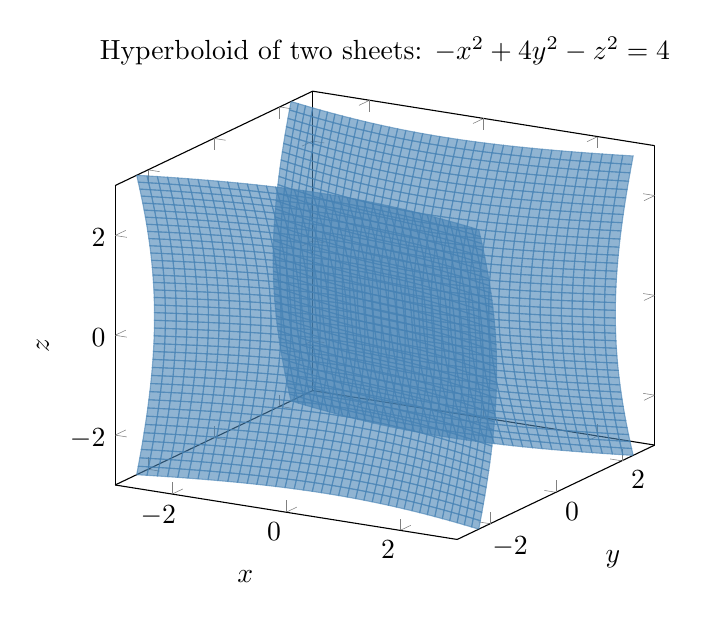
\begin{tikzpicture}
\begin{axis}[
    view={30}{20},
    xlabel=$x$, ylabel=$y$, zlabel=$z$,
    xmin=-3, xmax=3,
    ymin=-3, ymax=3,
    zmin=-3, zmax=3,
    samples=40,
    domain=-3:3,
    y domain=-3:3,
    colormap={steelblue}{rgb255=(70,130,180) rgb255=(70,130,180)},
    title={Hyperboloid of two sheets: $-x^2+4y^2-z^2=4$}
]
\addplot3[surf, opacity=0.6, shader=flat, draw=none, domain=-3:3, y domain=-3:3]
    ({x}, {sqrt(1+(x/2)^2+(y/2)^2)}, {y});
\addplot3[surf, opacity=0.6, shader=flat, draw=none, domain=-3:3, y domain=-3:3]
    ({x}, {-sqrt(1+(x/2)^2+(y/2)^2)}, {y});
\end{axis}
\end{tikzpicture}
\end{document}
